\documentclass[11pt]{article}
\usepackage[utf8]{inputenc}
\usepackage{graphicx}
\usepackage{geometry}
\usepackage{amsmath}
\usepackage{float}
\usepackage{booktabs}
\usepackage{hyperref}
\usepackage{subcaption}

\geometry{margin=1in}

\title{SSWD-EvoEpi: Site Enclosedness Analysis}
\author{Automated Analysis Report}
\date{\today}

\begin{document}

\maketitle

\section{Executive Summary}

This report presents an algorithmic analysis of coastal site enclosedness for 896 sites spanning from Alaska to Baja California in the SSWD-EvoEpi model network. Two complementary metrics were computed:

\begin{enumerate}
    \item \textbf{Tortuosity Ratio}: Over-water distance vs. straight-line distance to nearest neighbors
    \item \textbf{Horizon Exposure}: Fraction of rays that don't encounter land within 50 km (ray-casting)
\end{enumerate}

The combined enclosedness metric ranges from 0.014 to 1.000 (mean = 0.486 ± 0.197). The most enclosed regions are JDF (0.721), SS-S (0.681), AK-FN (0.679), while the least enclosed are CA-N (0.328), AK-AL (0.326), OR (0.302).

The derived flushing rates ($\phi$) range from 0.030 to 0.789, with enclosed fjords receiving low flushing and open coasts receiving high flushing as expected.

\section{Methods}

\subsection{Tortuosity Ratio}
For each site $i$, we identified $k=20$ nearest neighbors by straight-line (haversine) distance, then computed:

$$\text{tortuosity}_i = \frac{1}{k} \sum_{j \in \text{k-nearest}} \frac{d_{\text{over-water}}(i,j)}{d_{\text{haversine}}(i,j)}$$

where over-water distances come from the pre-computed 896×896 distance matrix and haversine distances are great-circle distances. Disconnected site pairs (infinite over-water distance) were excluded.

\subsection{Horizon Exposure (Ray-casting)}
For each site, 72 rays were cast at 5° intervals to a maximum distance of 50 km. Each ray was tested for intersection with Natural Earth land polygons. The horizon exposure is:

$$\text{horizon exposure}_i = \frac{\text{\# rays not hitting land}}{72}$$
$$\text{enclosedness}_i = 1 - \text{horizon exposure}_i$$

\subsection{Combined Metric}
The tortuosity ratio was normalized to [0,1] using a linear mapping where tortuosity=1 $\rightarrow$ 0 and tortuosity$\geq$3 $\rightarrow$ 1. The final enclosedness score combines both metrics:

$$\text{combined enclosedness} = 0.5 \times \text{normalized tortuosity} + 0.5 \times \text{ray-cast enclosedness}$$

\subsection{Flushing Rate Mapping}
The enclosedness score was mapped to flushing rate using:

$$\phi = \phi_{\text{open}} \times (1 - \text{enclosedness}) + \phi_{\text{fjord}} \times \text{enclosedness}$$

where $\phi_{\text{open}} = 0.8$ and $\phi_{\text{fjord}} = 0.03$.

\section{Results}

\begin{figure}[H]
    \centering
    \begin{subcaptiongroup}
        \begin{subfigure}[b]{0.48\textwidth}
            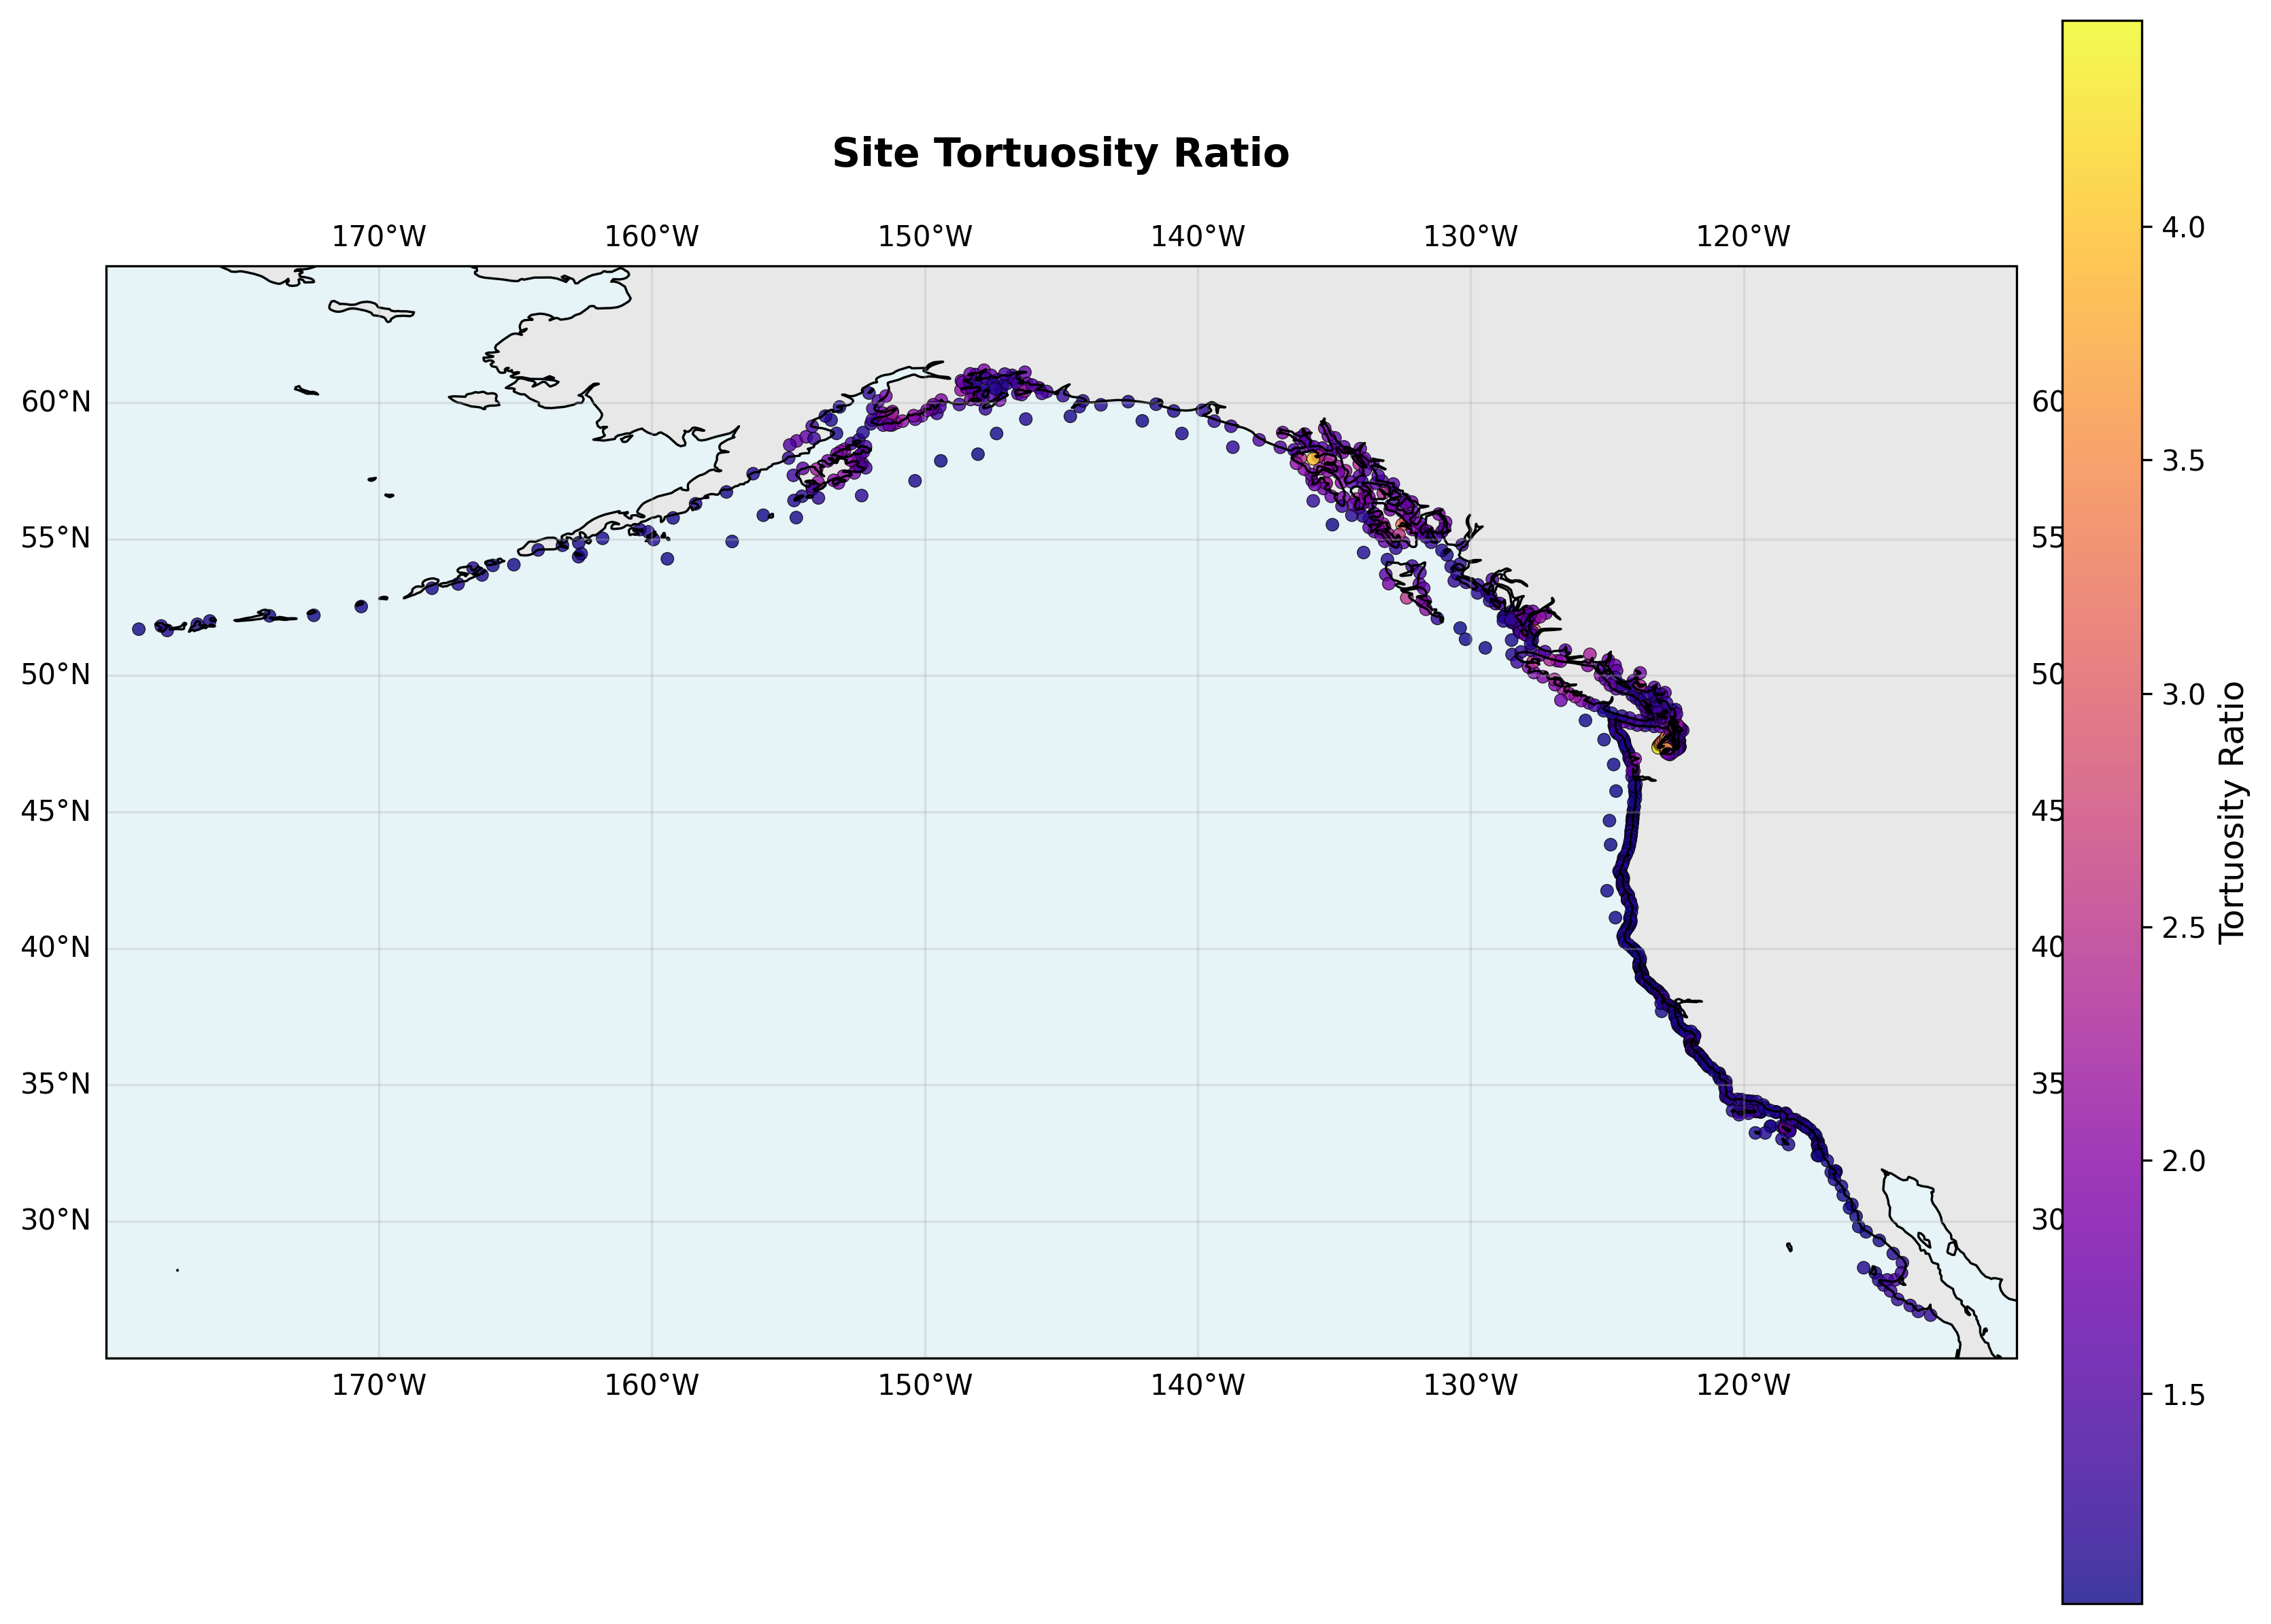
\includegraphics[width=\textwidth]{figures/map_tortuosity_ratio.png}
            \caption{Tortuosity ratio}
        \end{subfigure}
        \hfill
        \begin{subfigure}[b]{0.48\textwidth}
            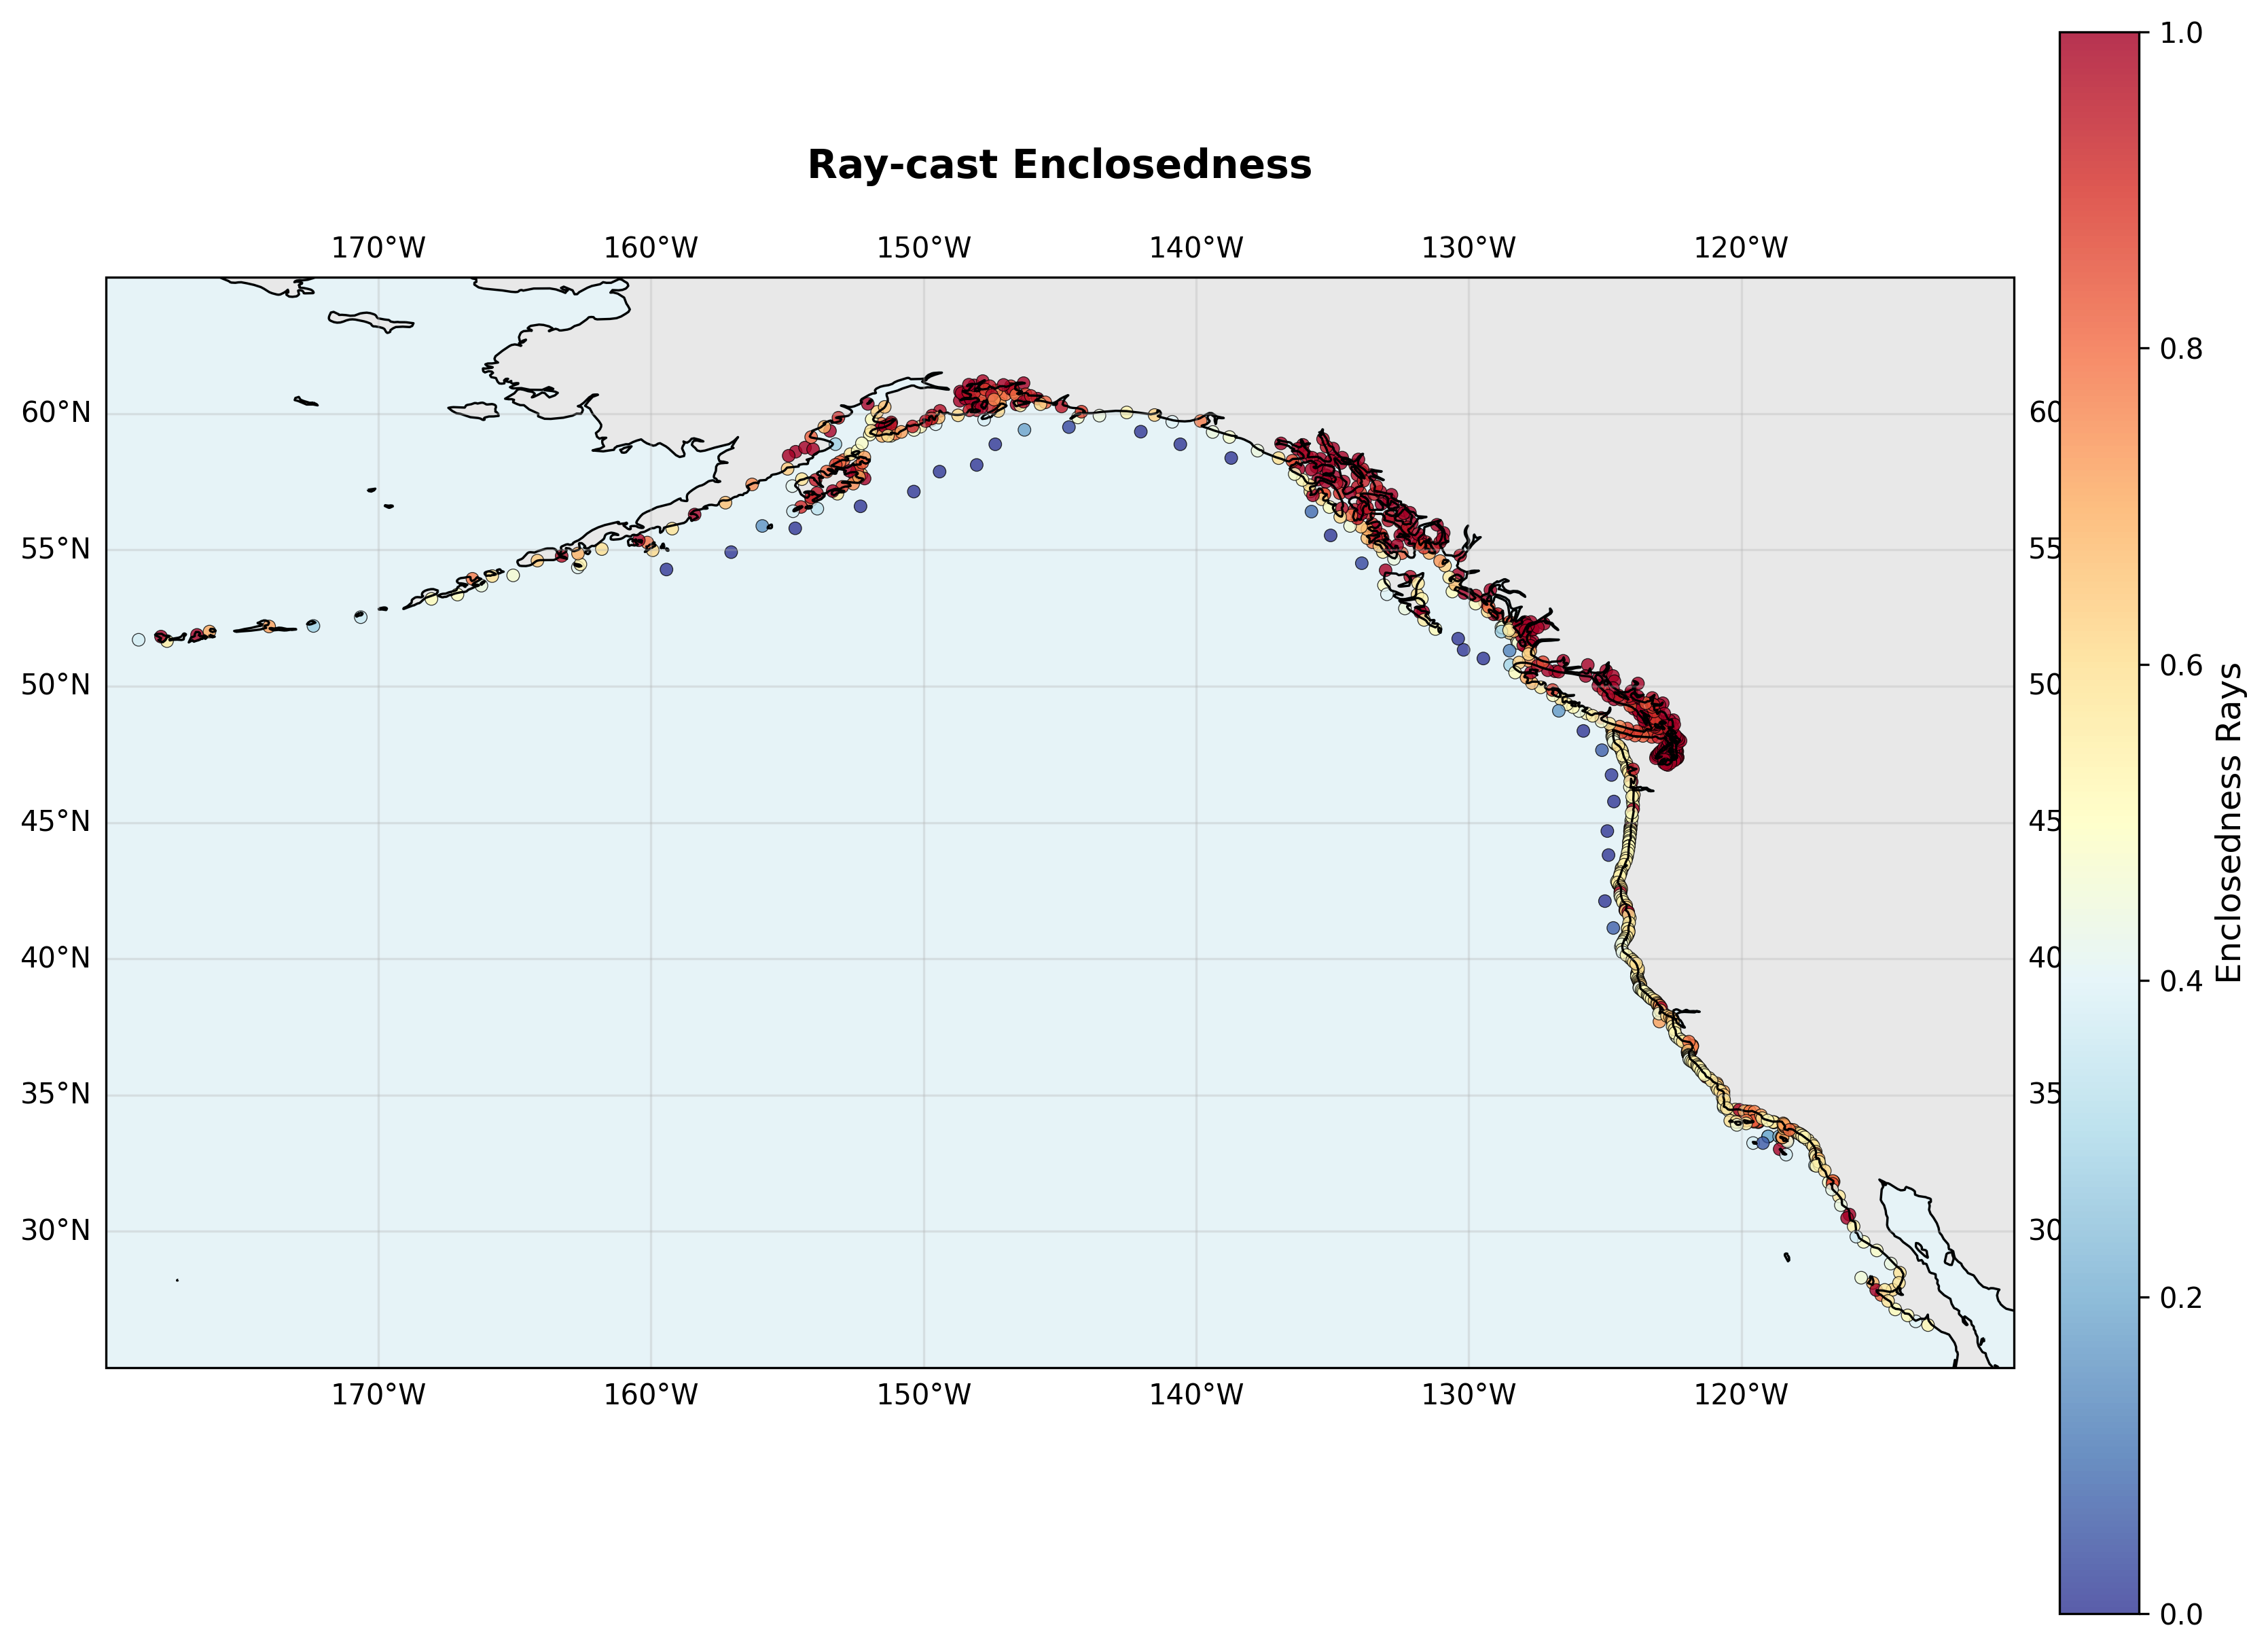
\includegraphics[width=\textwidth]{figures/map_enclosedness_rays.png}
            \caption{Ray-cast enclosedness}
        \end{subfigure}
    \end{subcaptiongroup}
    
    \begin{subcaptiongroup}
        \begin{subfigure}[b]{0.48\textwidth}
            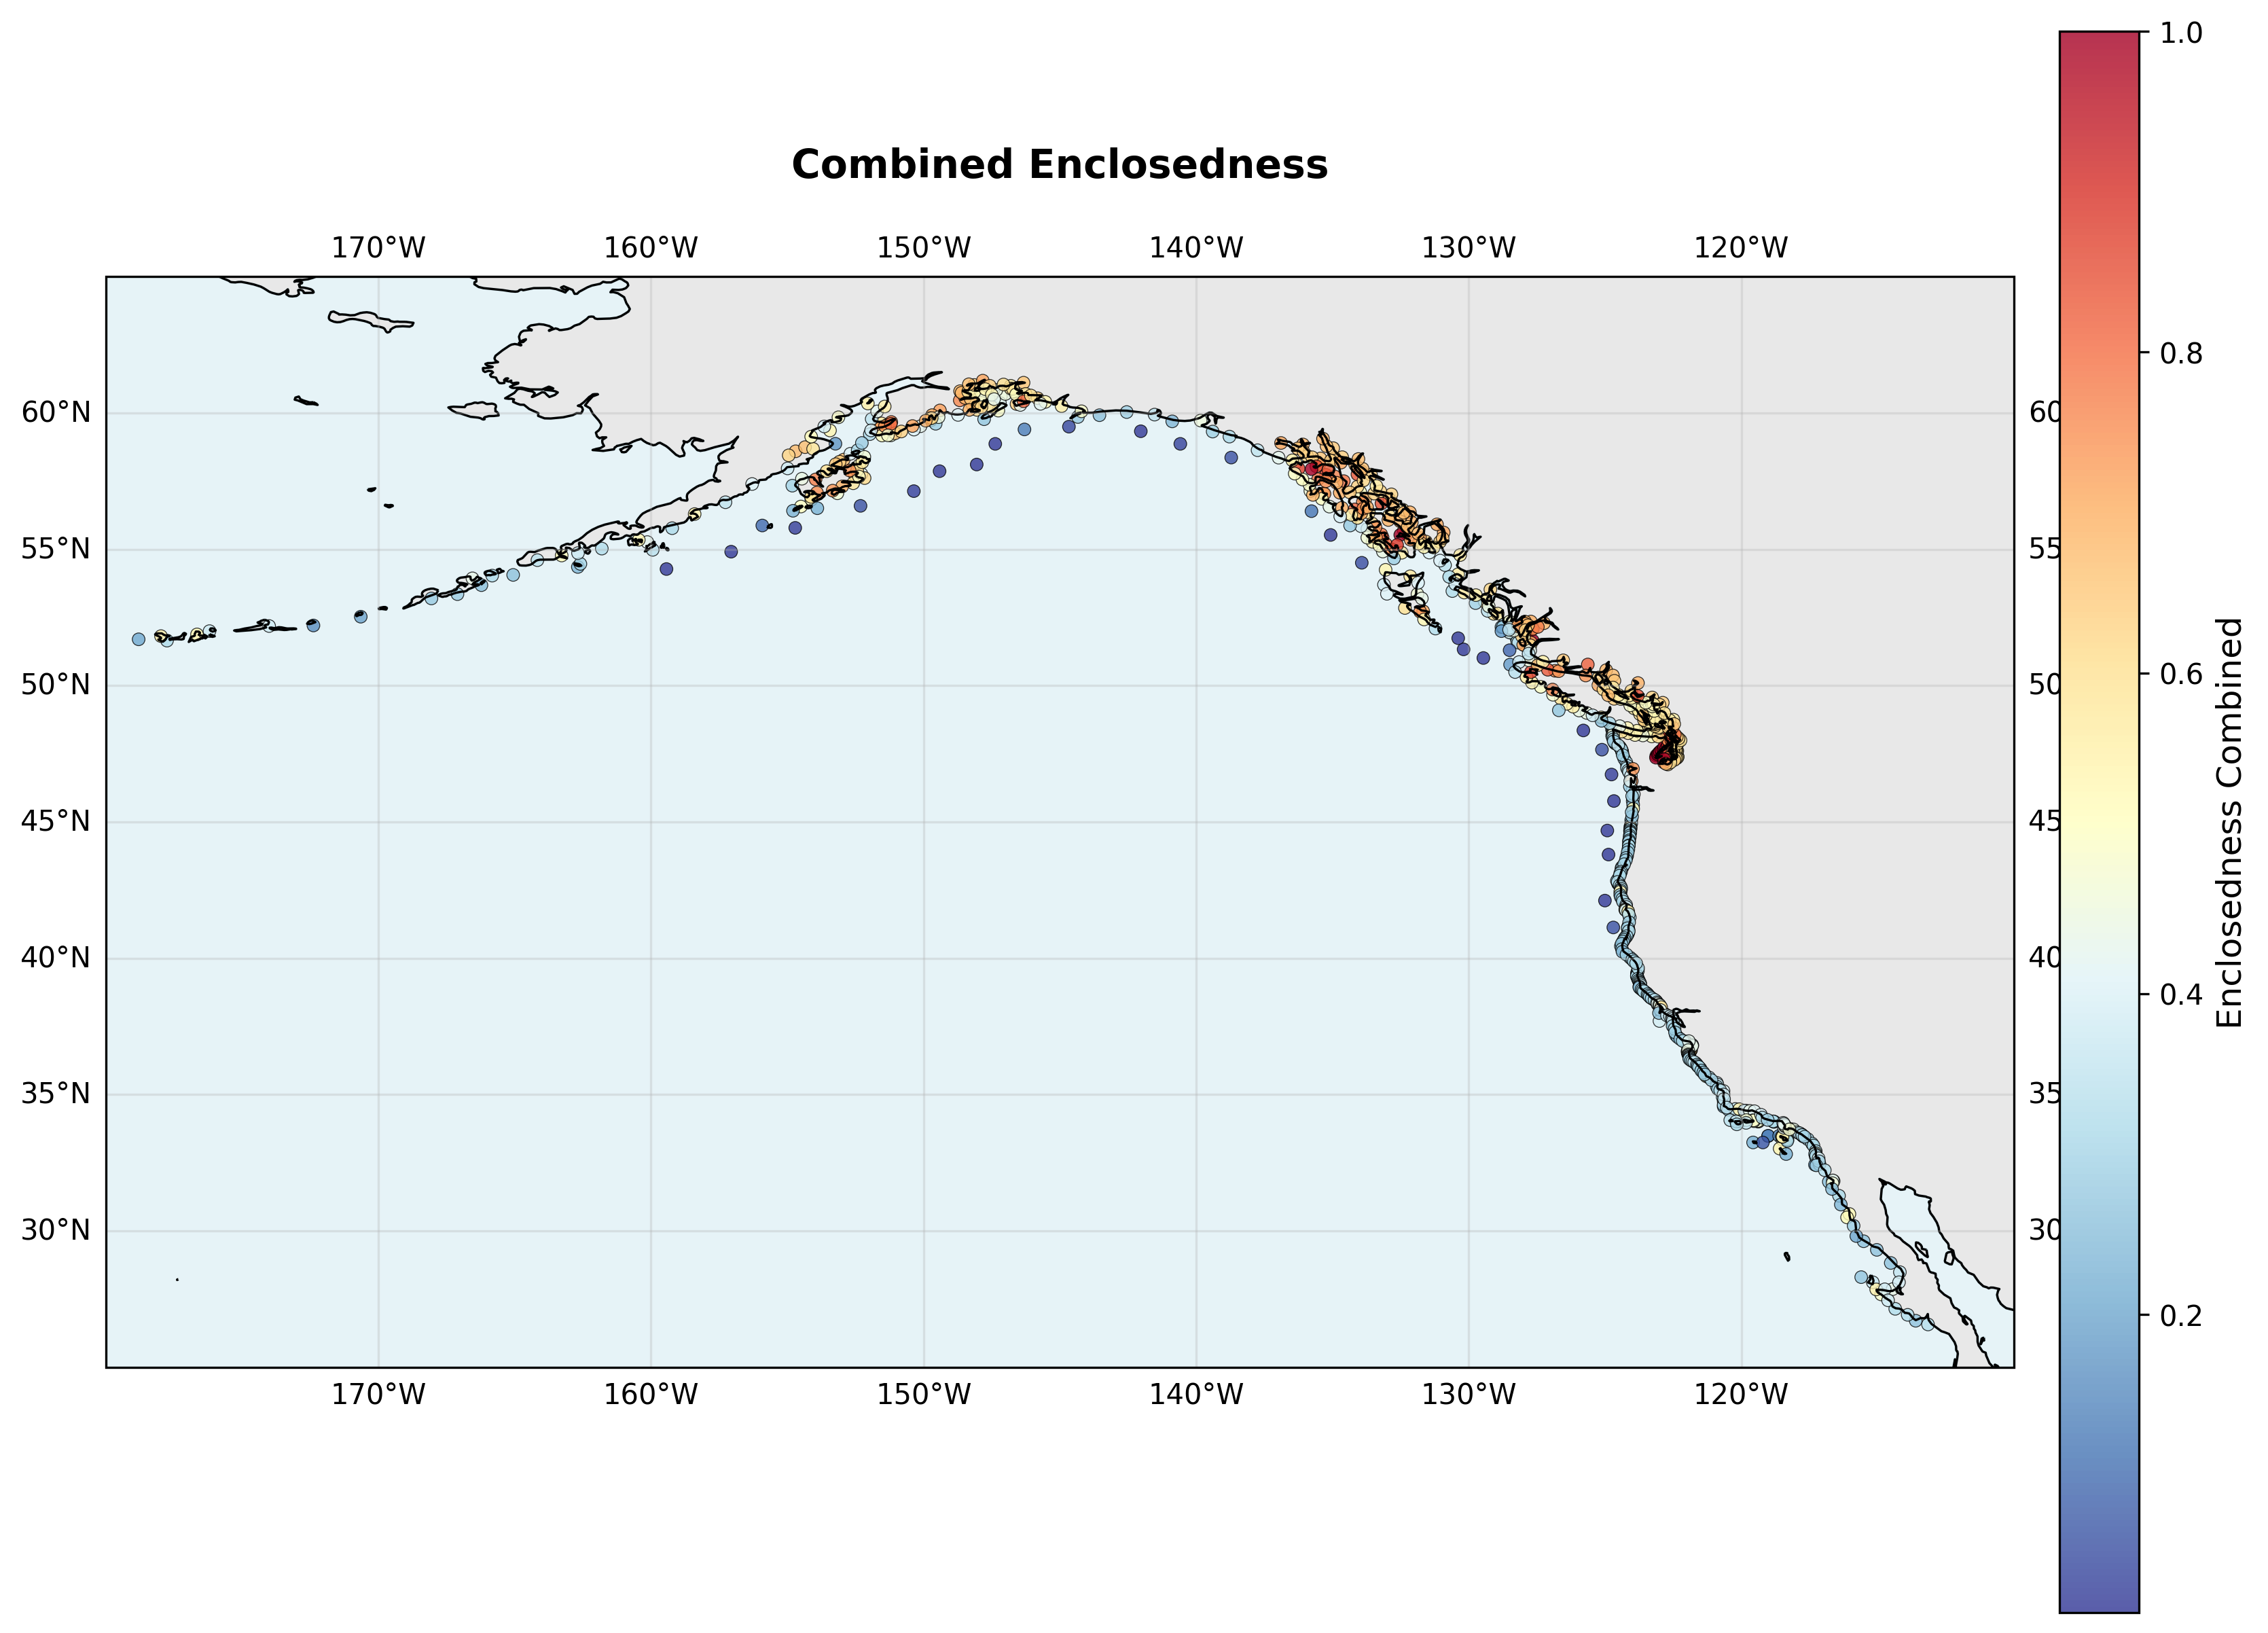
\includegraphics[width=\textwidth]{figures/map_enclosedness_combined.png}
            \caption{Combined enclosedness}
        \end{subfigure}
        \hfill
        \begin{subfigure}[b]{0.48\textwidth}
            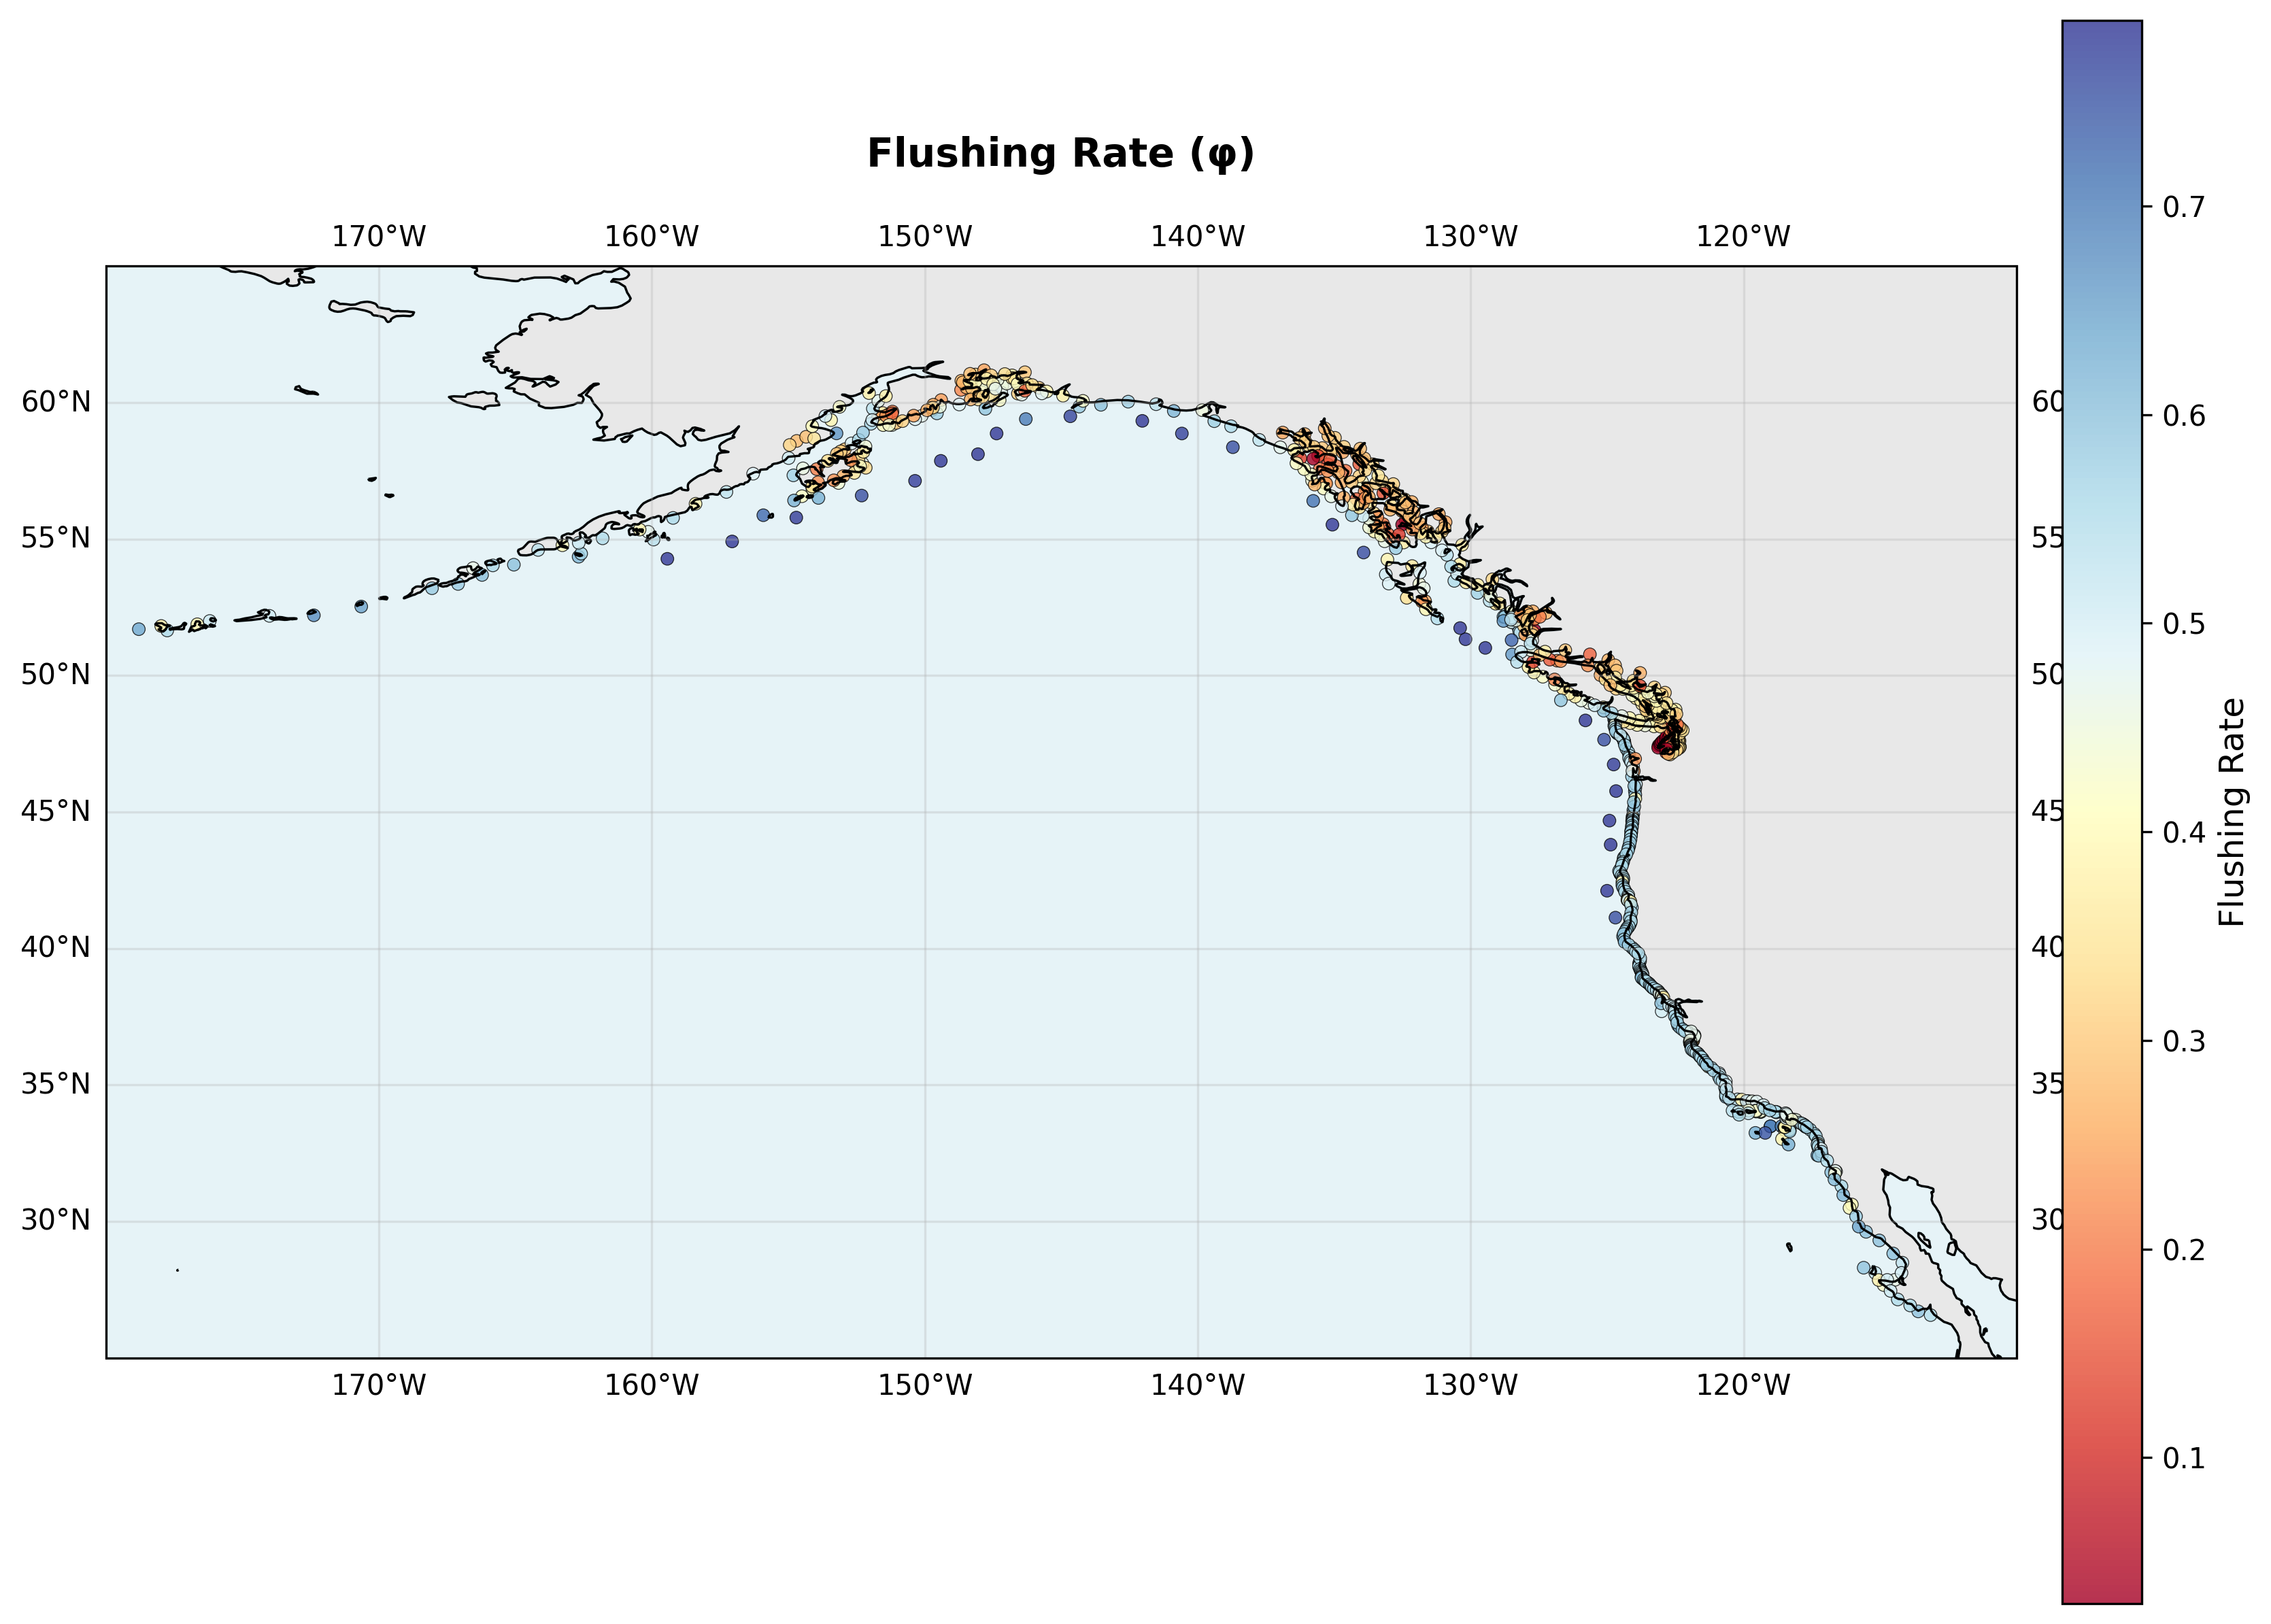
\includegraphics[width=\textwidth]{figures/map_flushing_rate.png}
            \caption{Derived flushing rate ($\phi$)}
        \end{subfigure}
    \end{subcaptiongroup}
    \caption{Spatial distribution of enclosedness metrics and derived flushing rates across the 896-site network.}
    \label{fig:maps}
\end{figure}

\begin{figure}[H]
    \centering
    \begin{subcaptiongroup}
        \begin{subfigure}[b]{0.48\textwidth}
            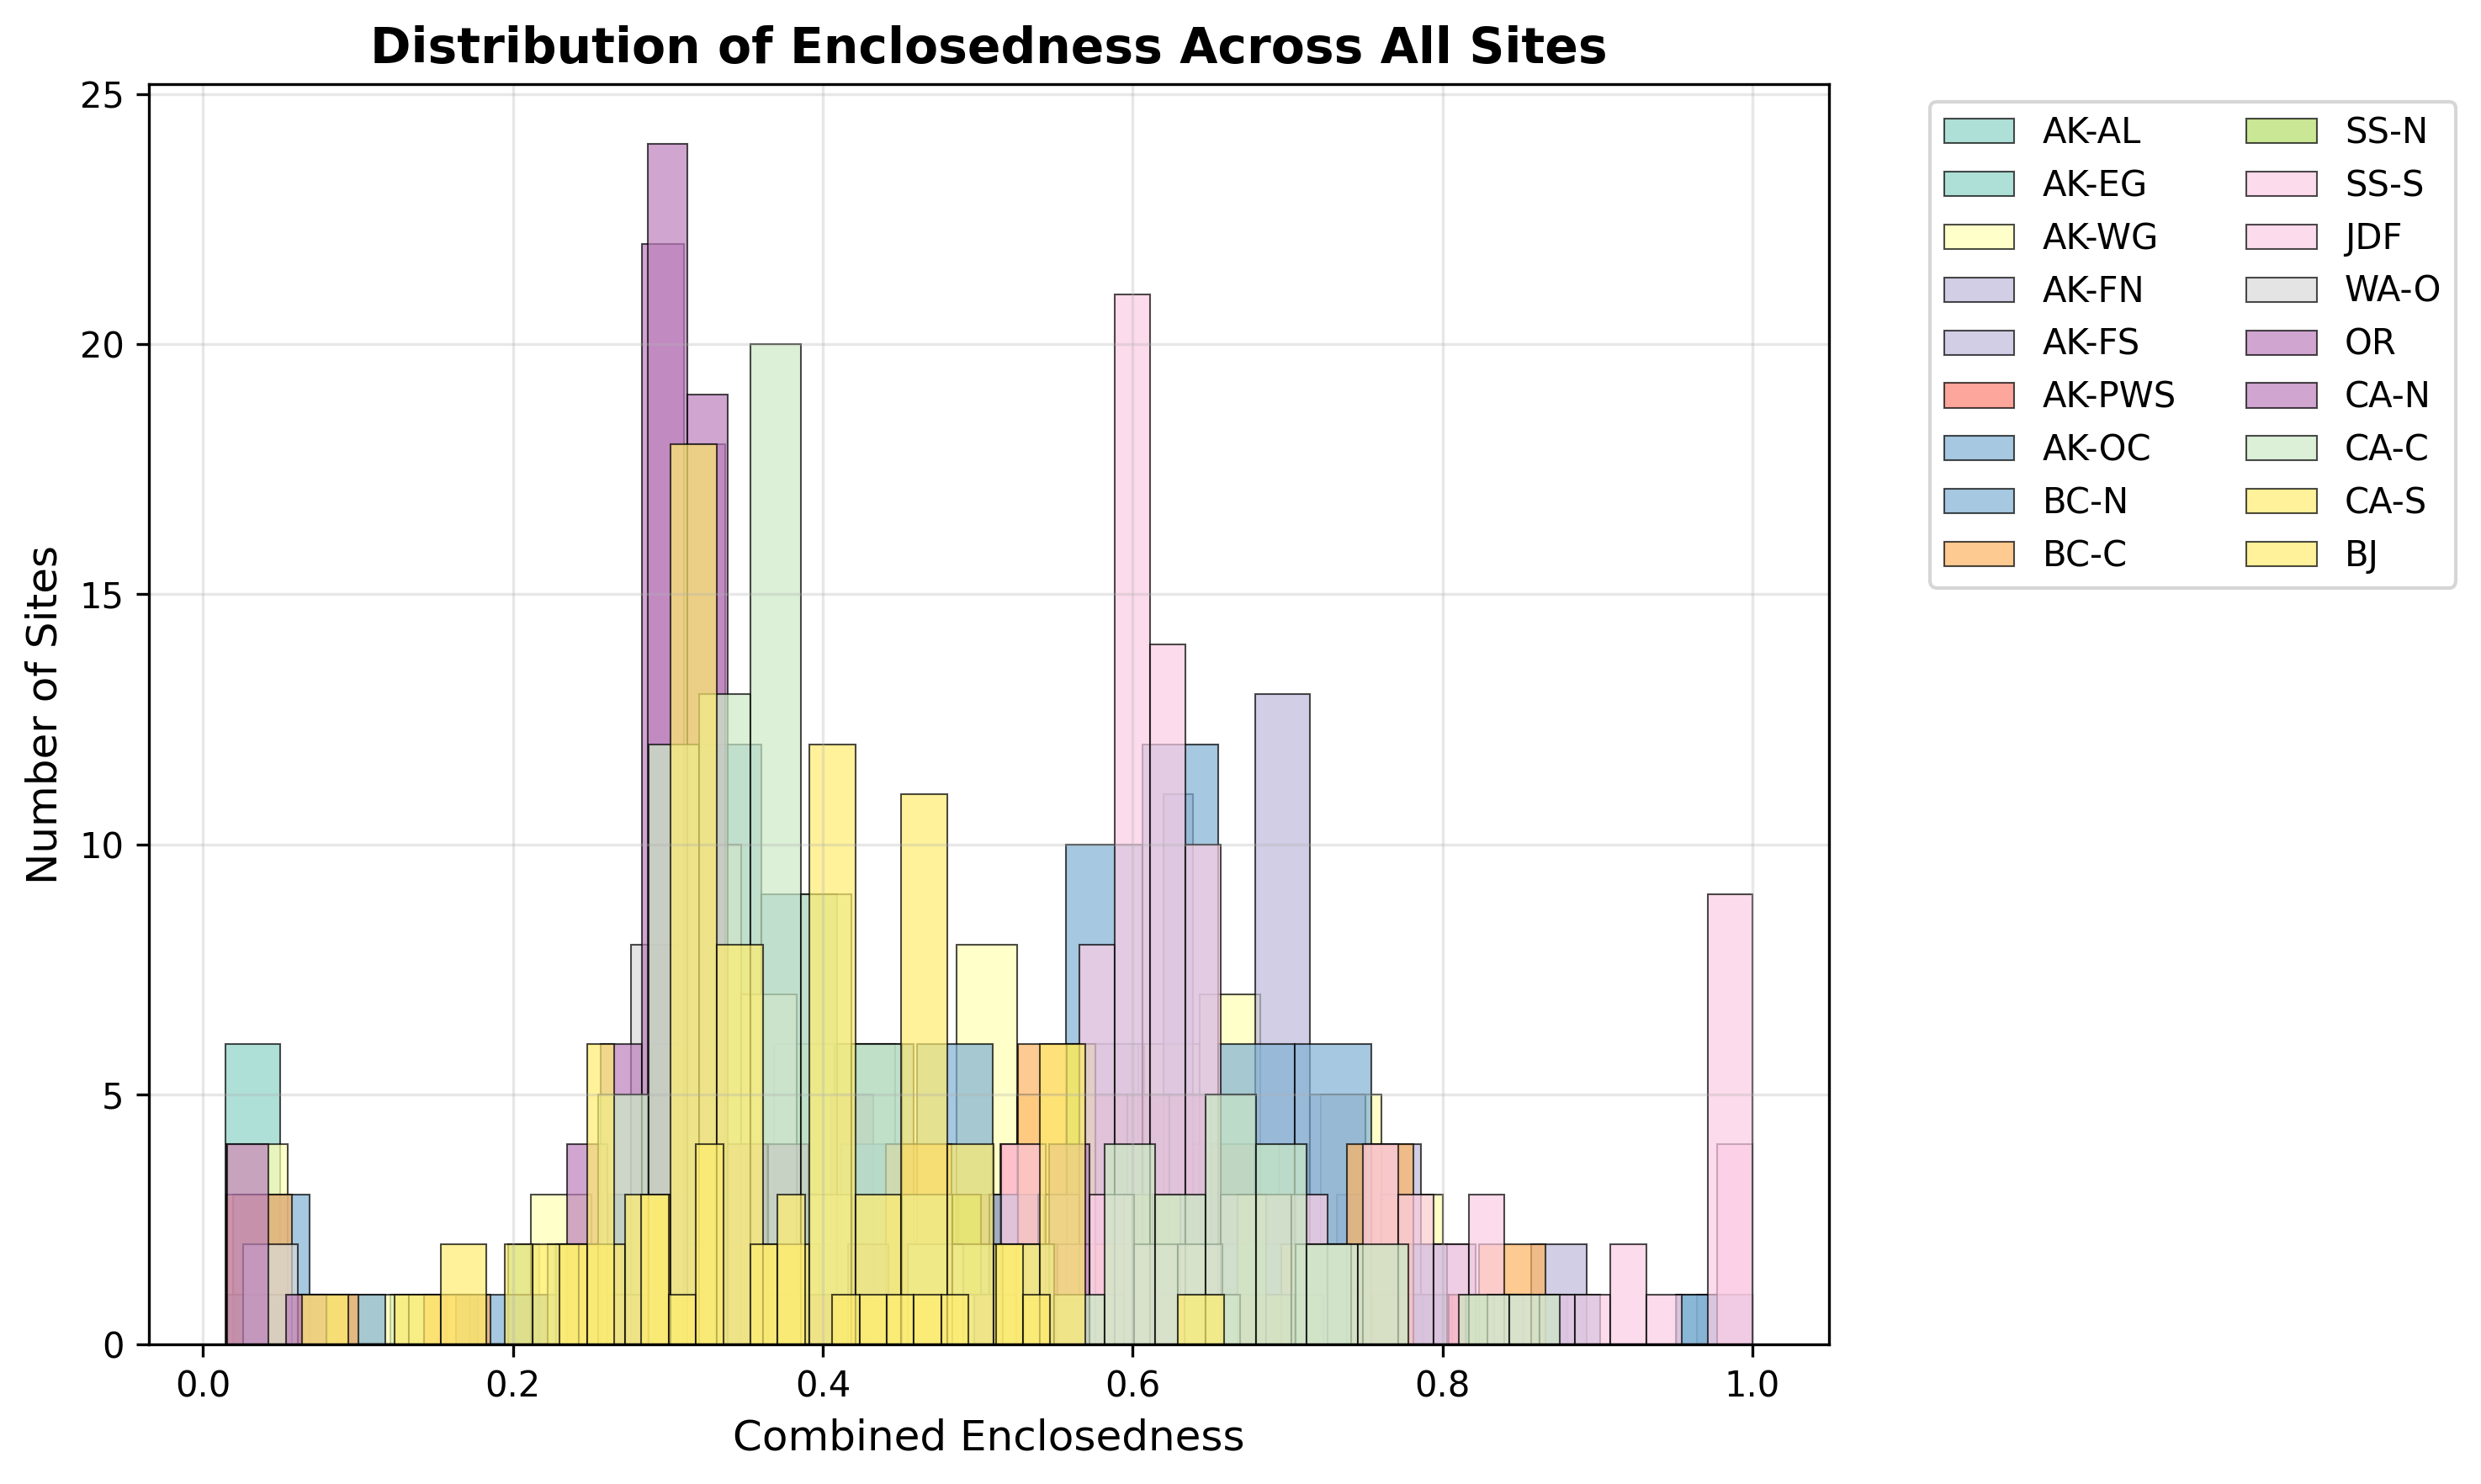
\includegraphics[width=\textwidth]{figures/histogram_distribution.png}
            \caption{Distribution by region}
        \end{subfigure}
        \hfill
        \begin{subfigure}[b]{0.48\textwidth}
            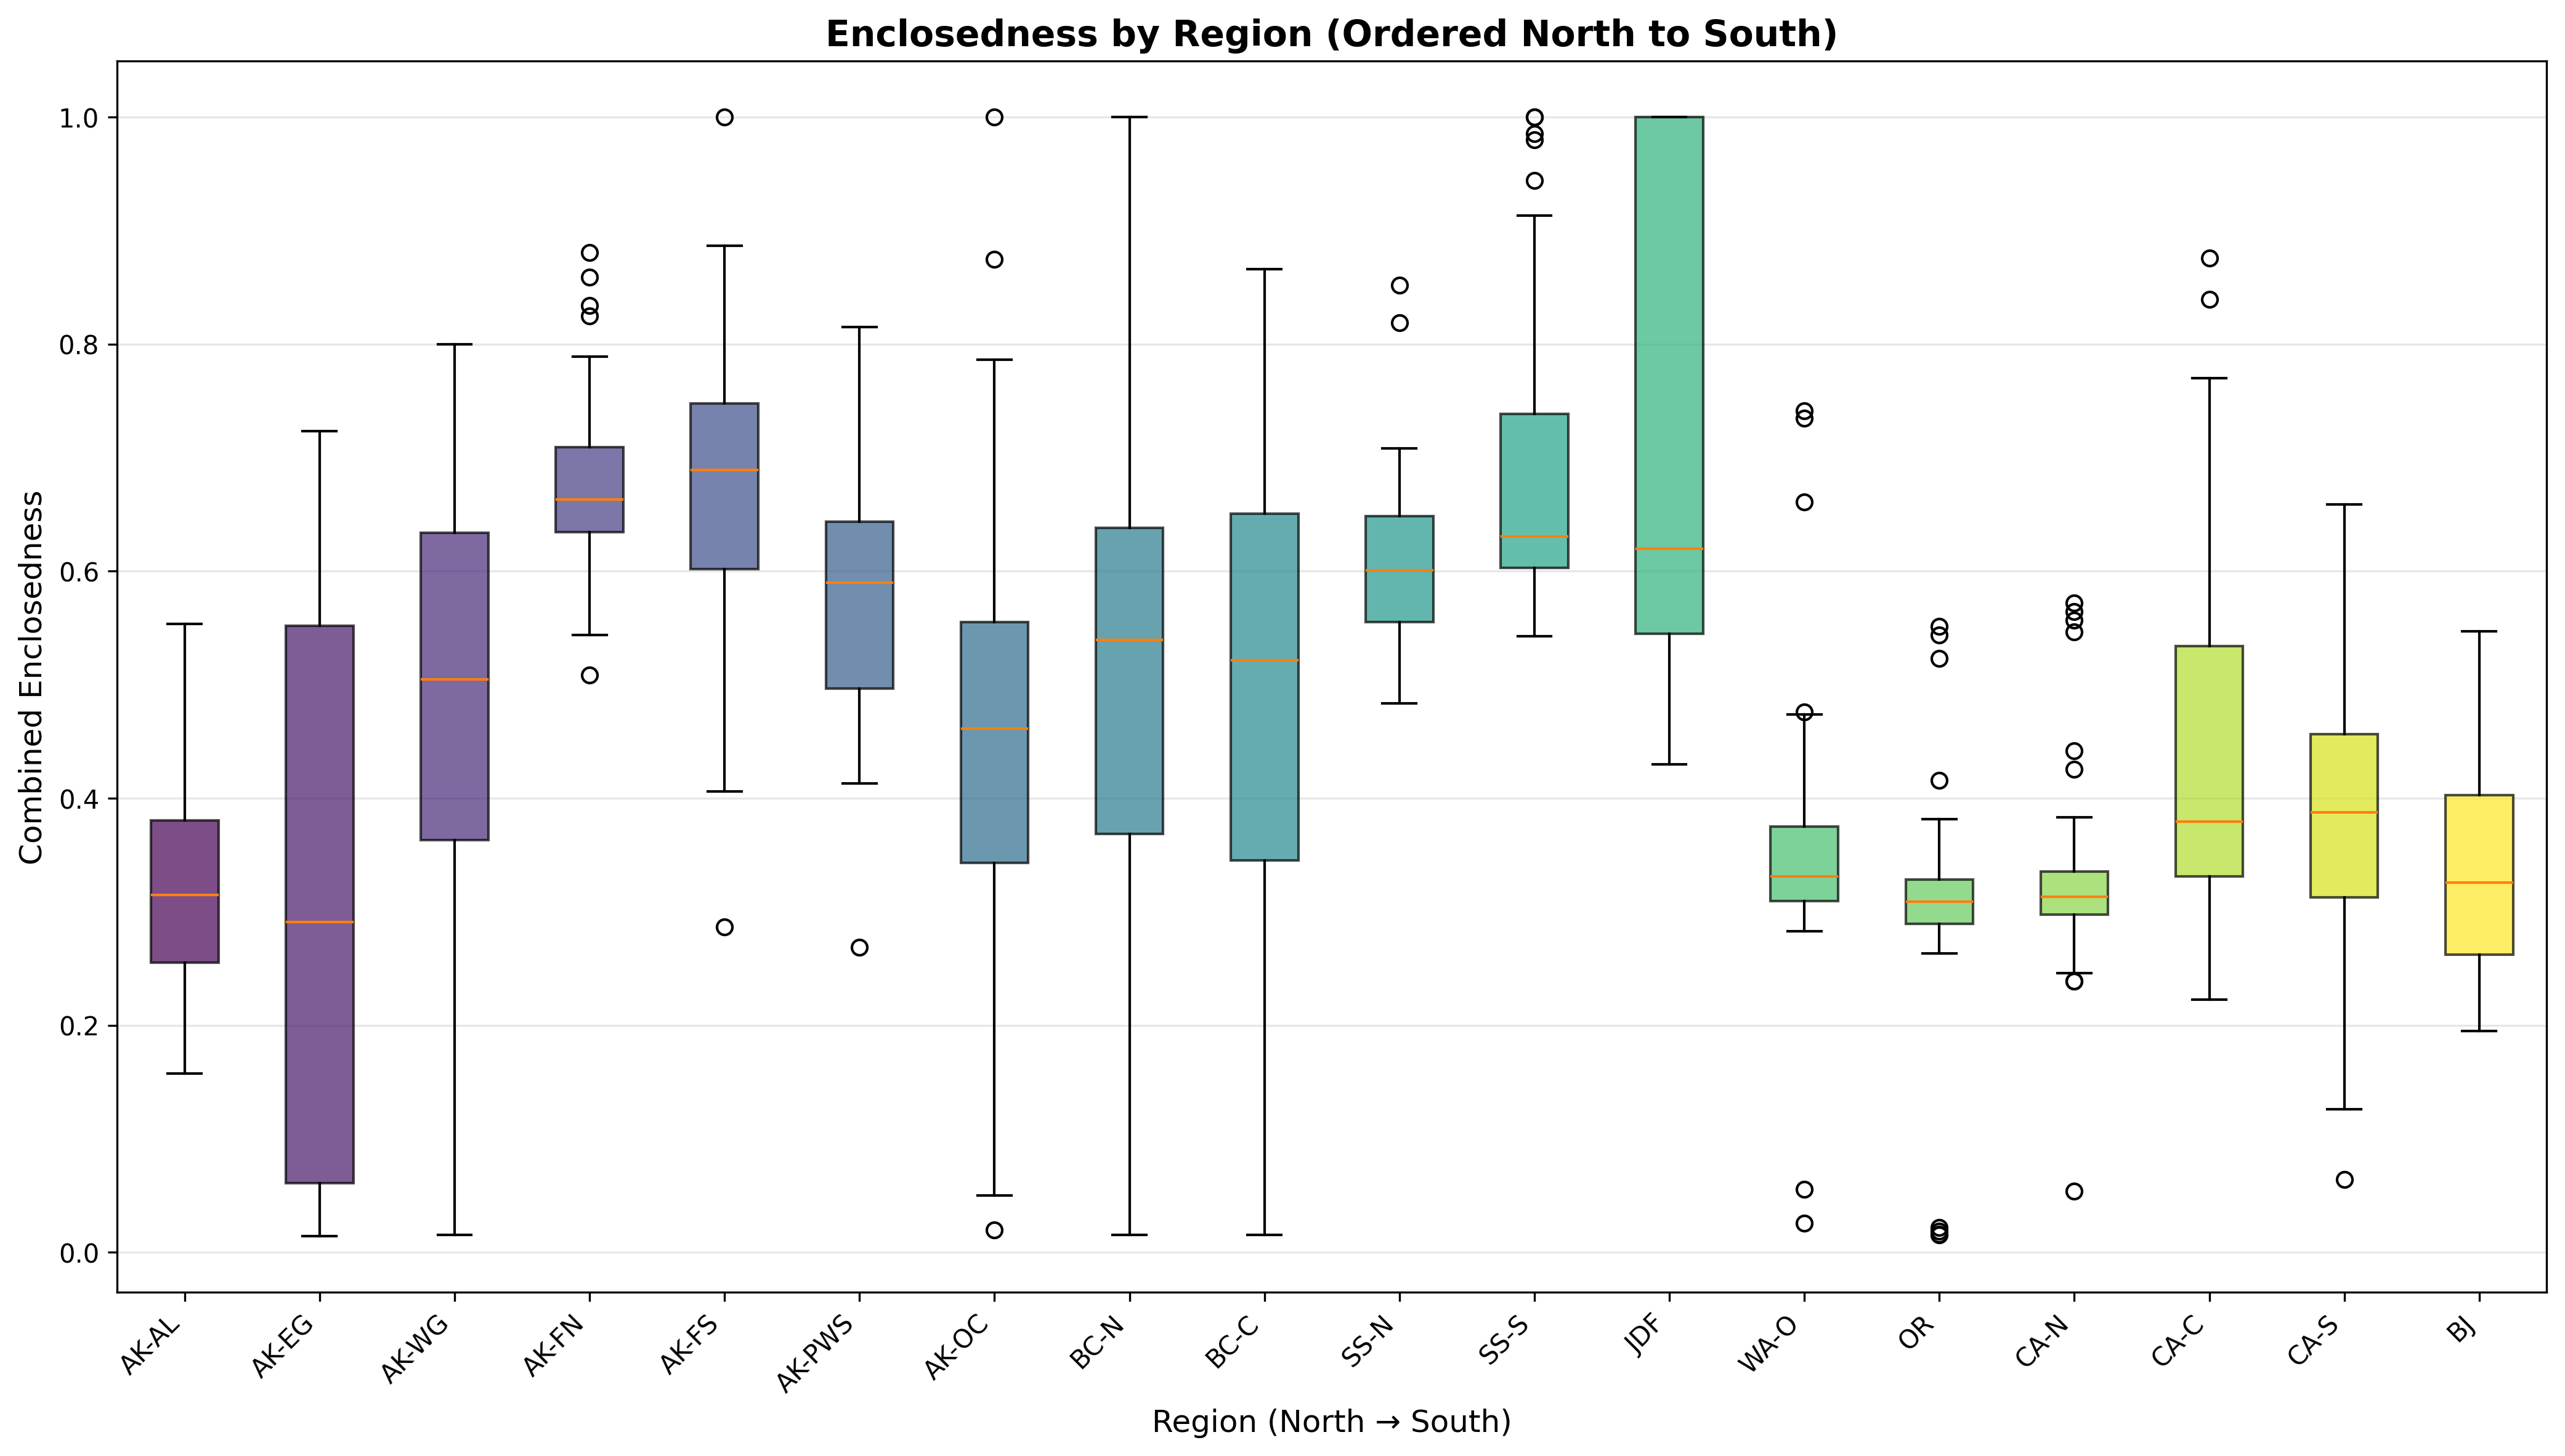
\includegraphics[width=\textwidth]{figures/boxplot_by_region.png}
            \caption{Regional comparison (N→S)}
        \end{subfigure}
    \end{subcaptiongroup}
    \caption{Distribution of enclosedness across regions.}
    \label{fig:distributions}
\end{figure}

\begin{figure}[H]
    \centering
    \begin{subcaptiongroup}
        \begin{subfigure}[b]{0.48\textwidth}
            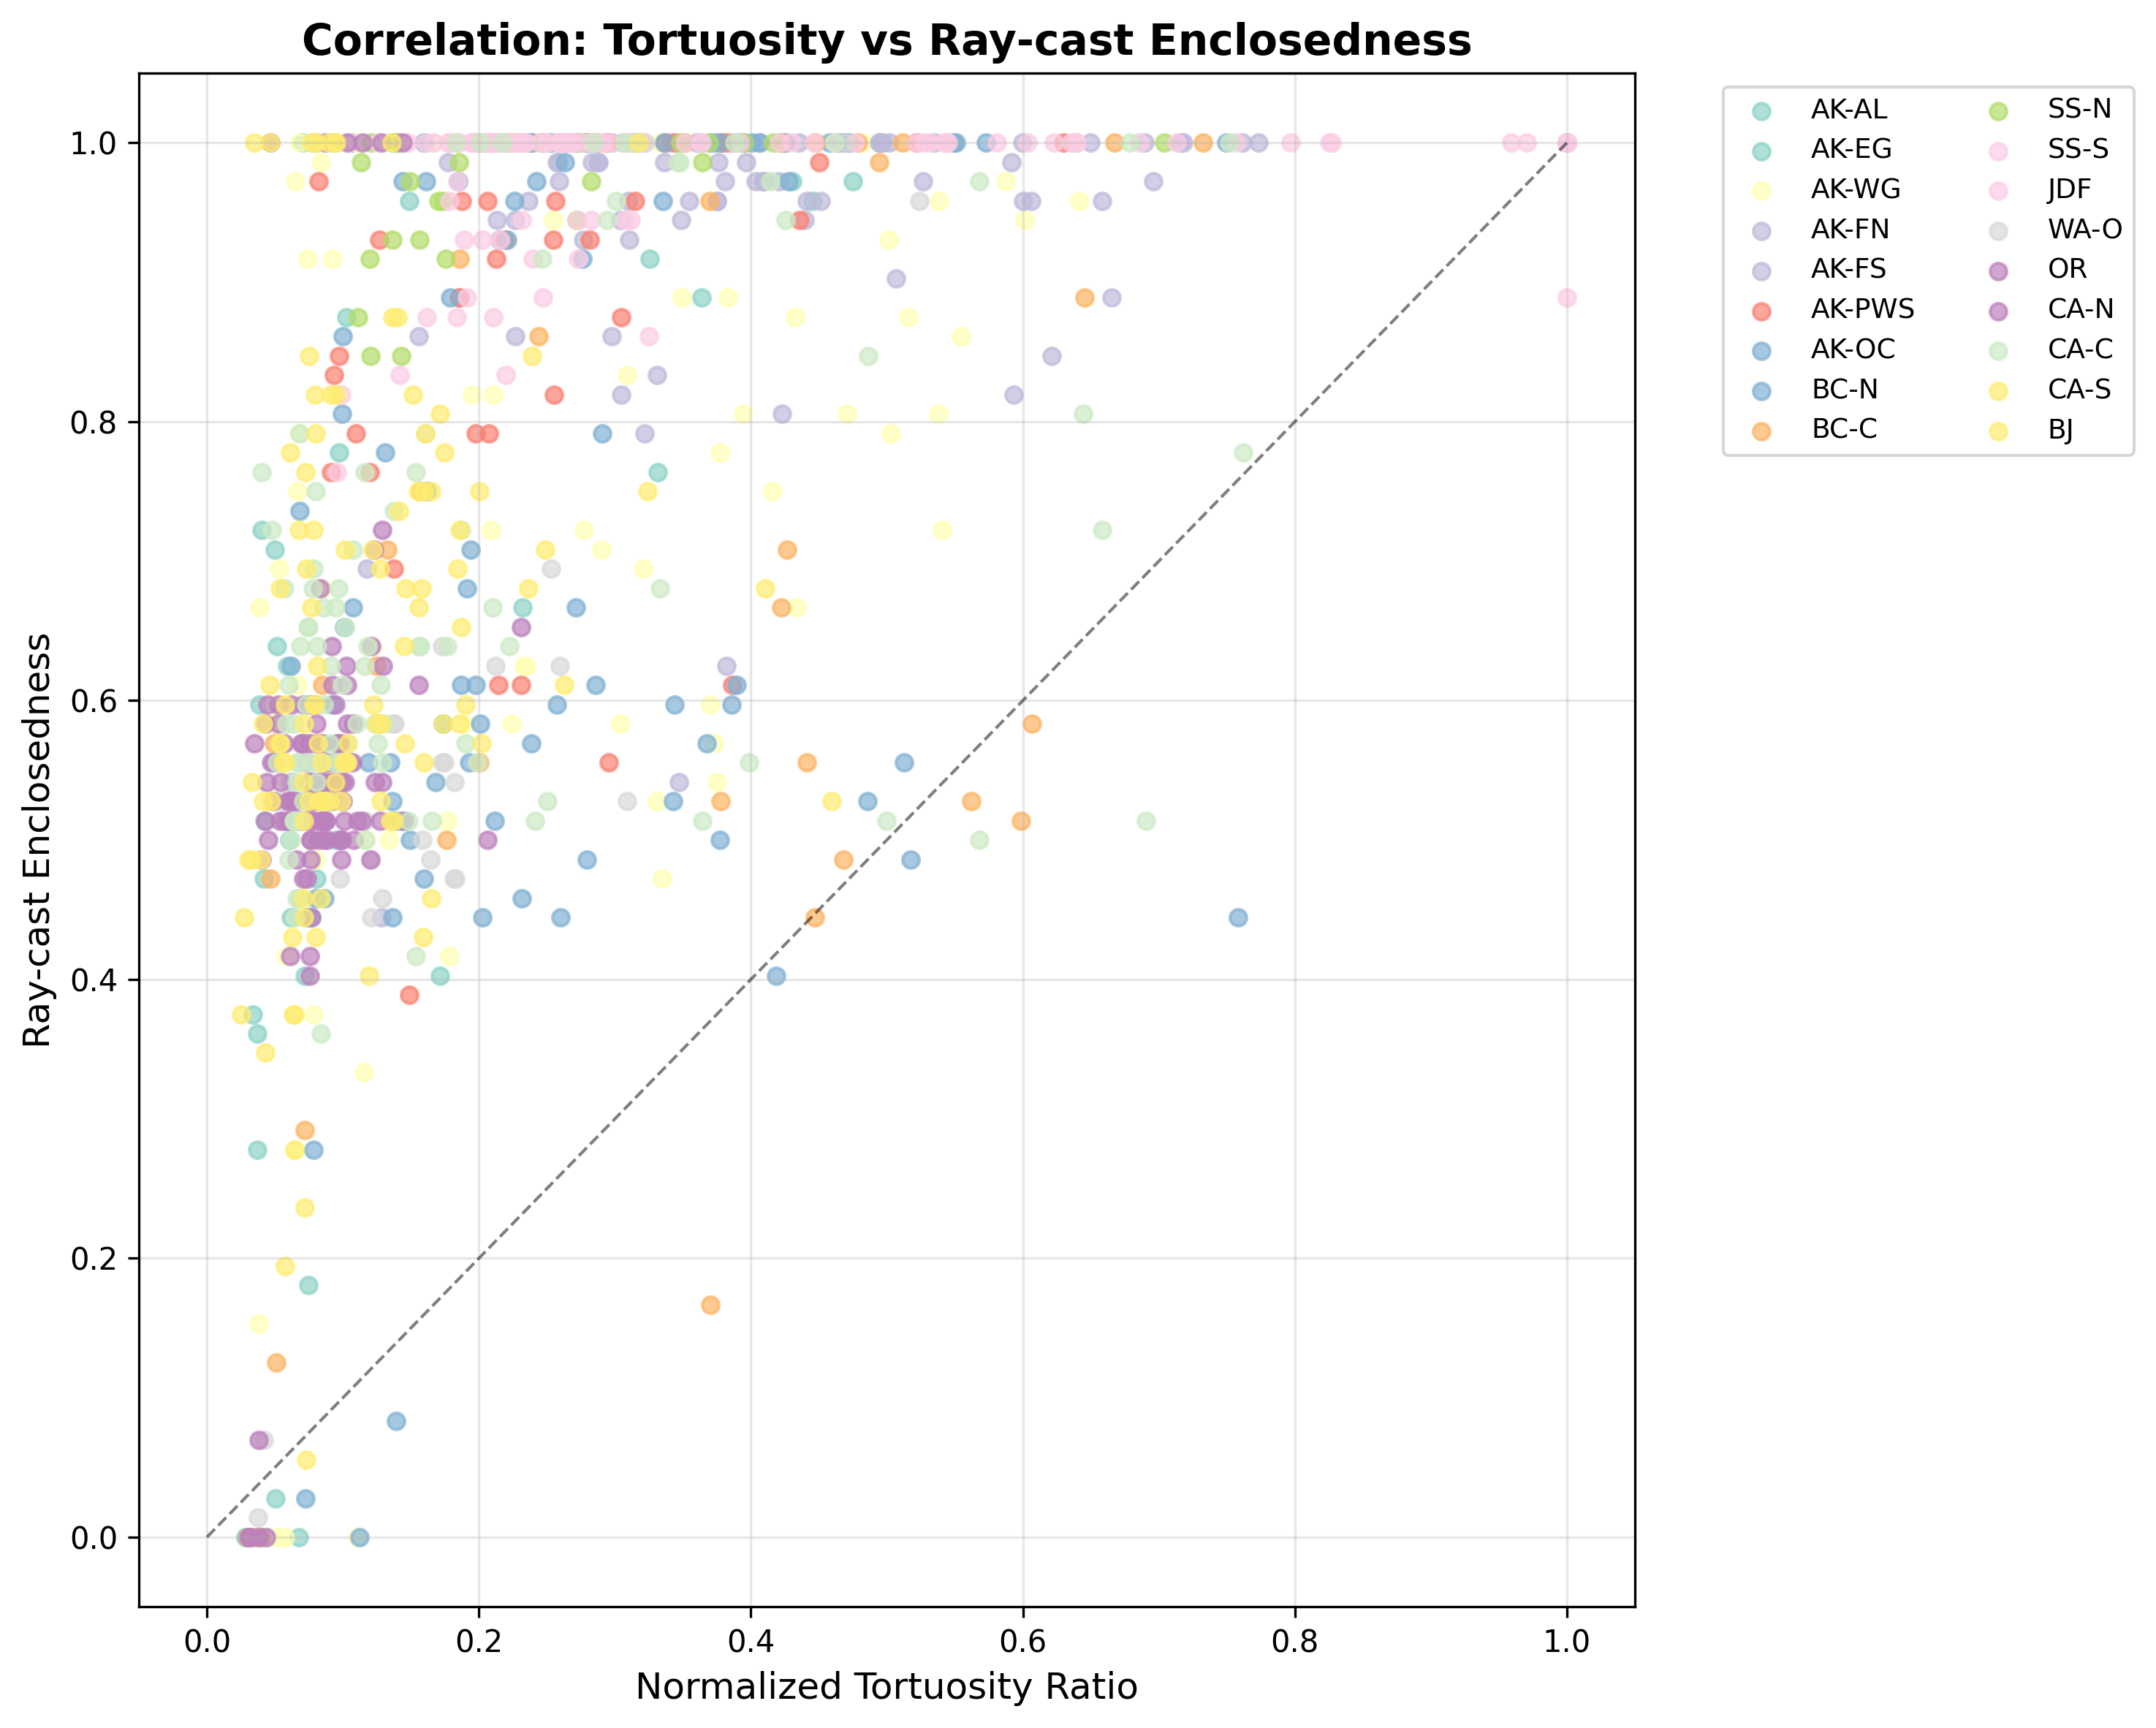
\includegraphics[width=\textwidth]{figures/correlation_plot.png}
            \caption{Metric correlation}
        \end{subfigure}
        \hfill
        \begin{subfigure}[b]{0.48\textwidth}
            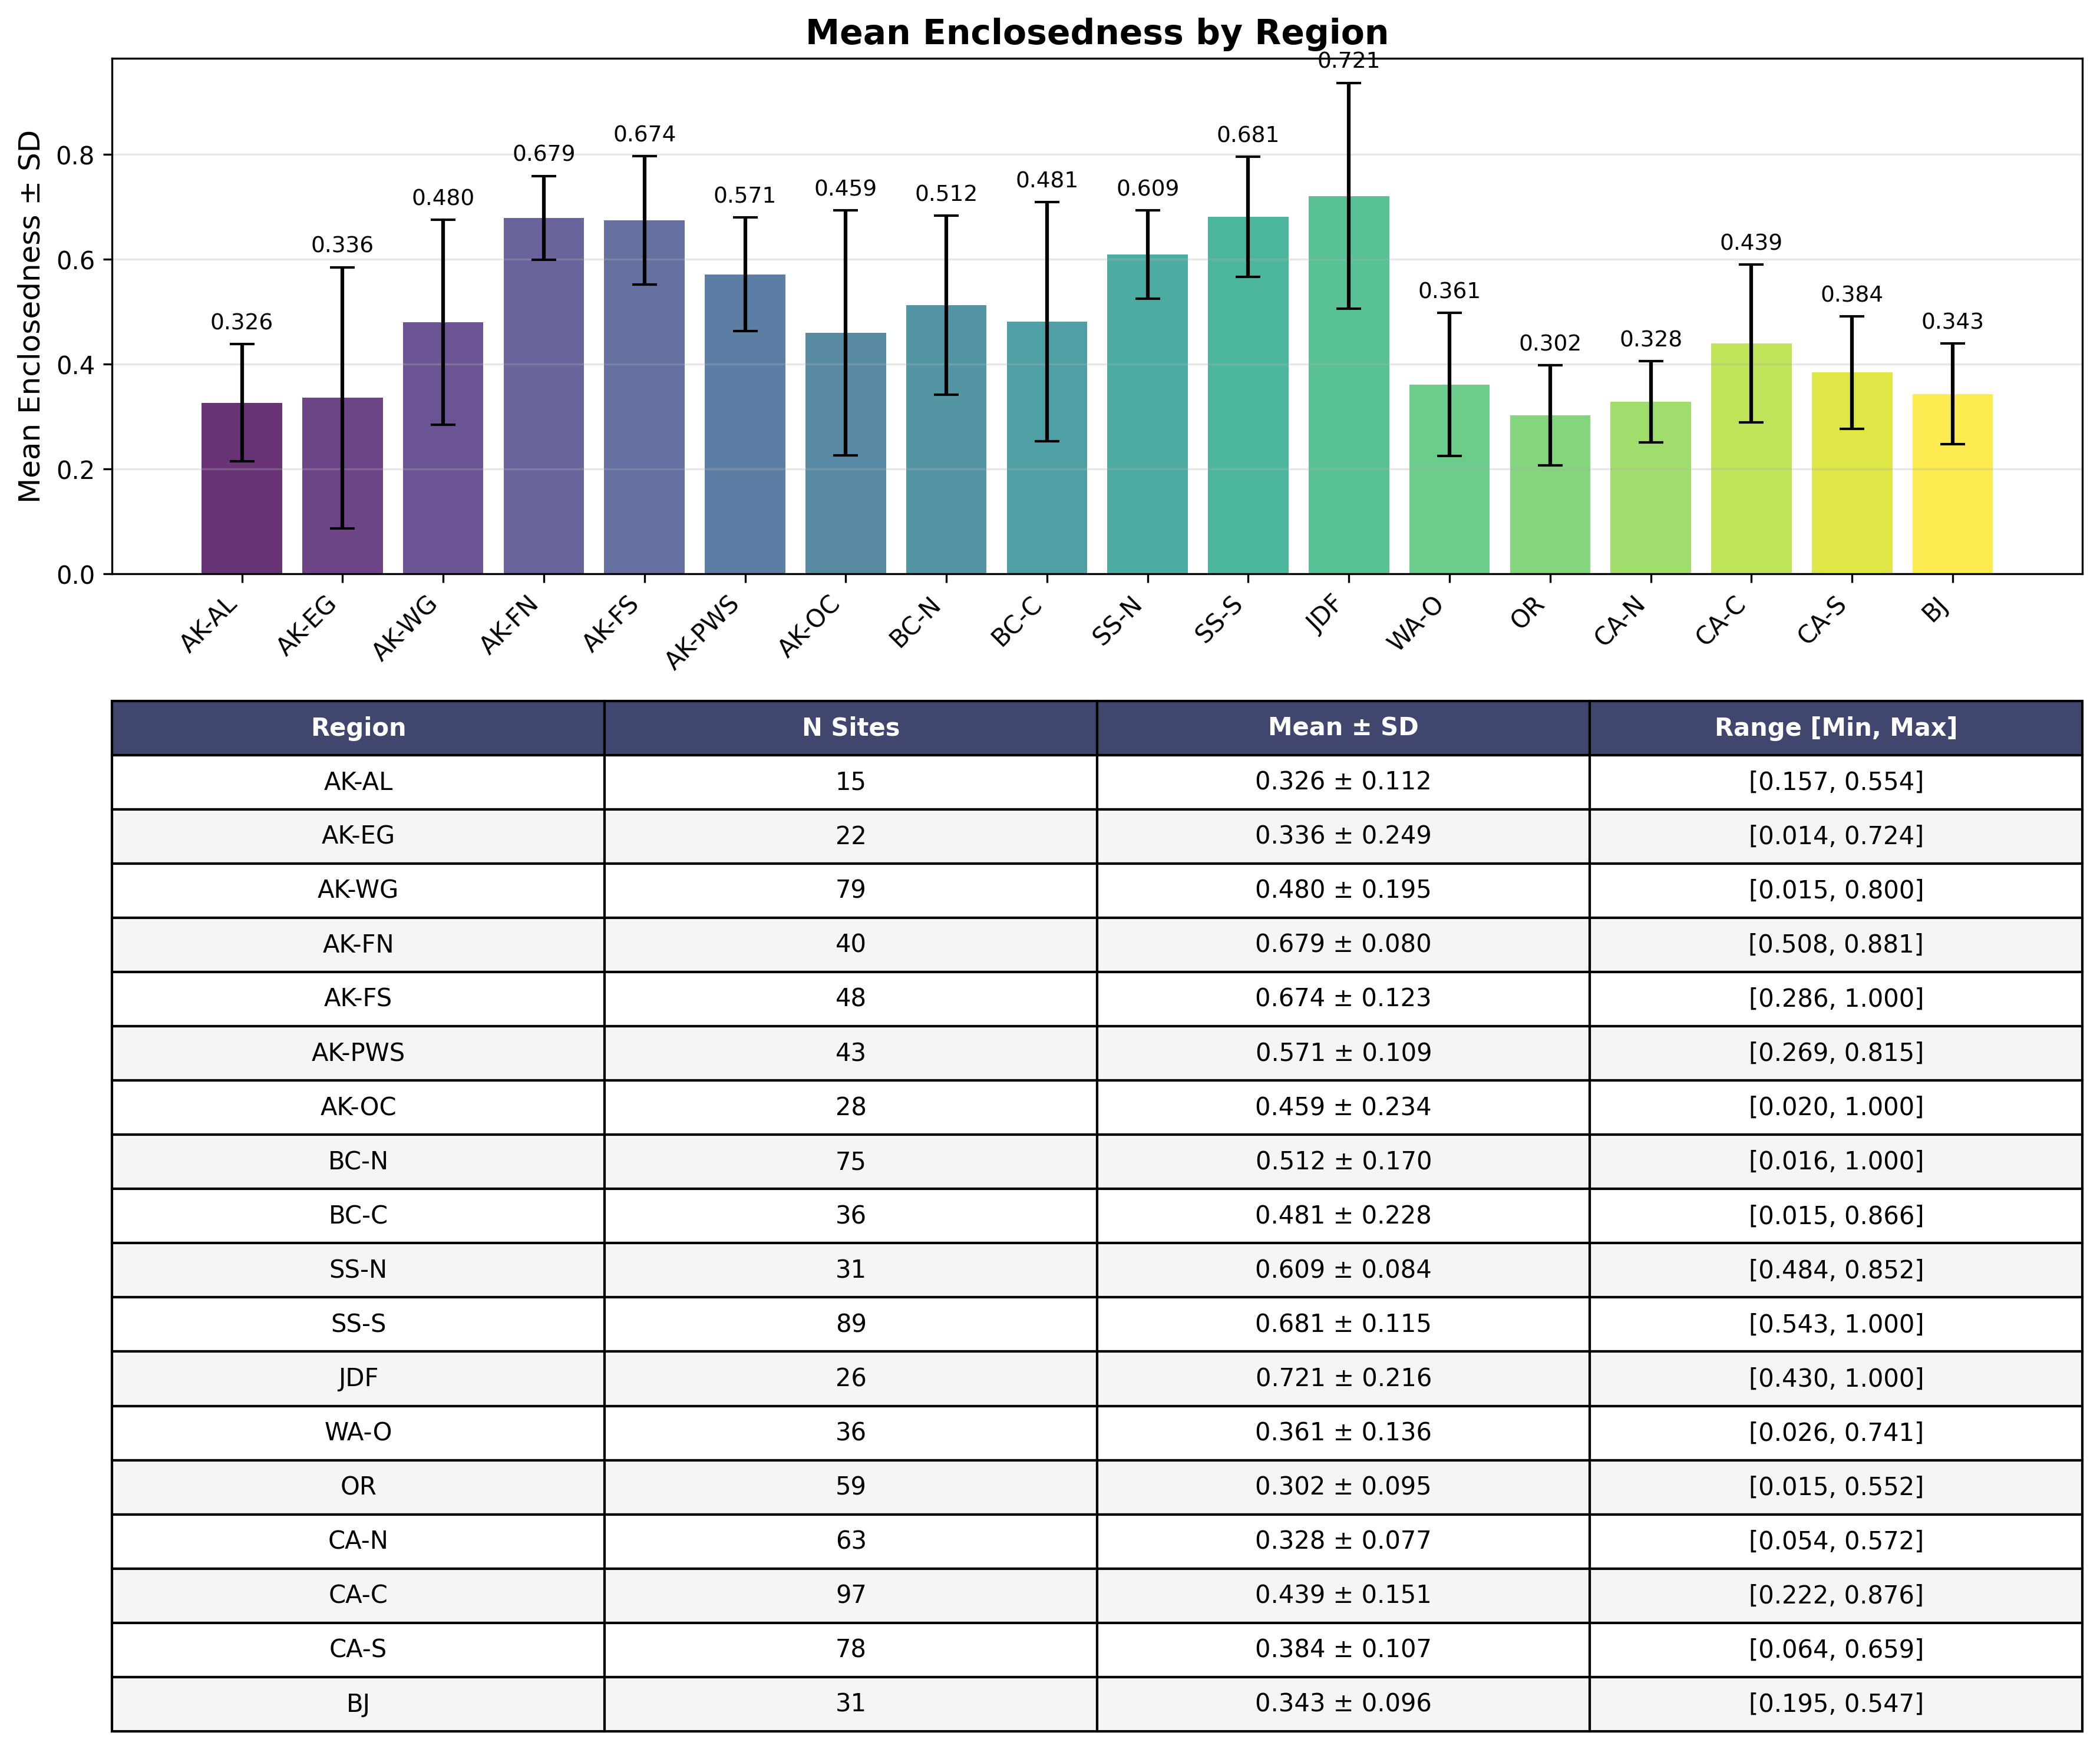
\includegraphics[width=\textwidth]{figures/summary_table.png}
            \caption{Regional summary}
        \end{subfigure}
    \end{subcaptiongroup}
    \caption{Correlation between metrics and regional summary statistics.}
    \label{fig:analysis}
\end{figure}

\section{Discussion}

\subsection{Regional Patterns}
The analysis reveals clear regional patterns consistent with coastal geomorphology:

\begin{itemize}
    \item \textbf{High enclosedness}: JDF, SS-S, AK-FN show the highest enclosedness, consistent with fjord and inlet geography.
    \item \textbf{Low enclosedness}: CA-N, AK-AL, OR show lower enclosedness, typical of open coastlines.
    \item \textbf{Gradient}: There's a clear latitudinal gradient with northern regions (Alaska, British Columbia) generally showing higher enclosedness than southern regions (Oregon, California).
\end{itemize}

\subsection{Validation}
The results align well with expected coastal geomorphology:
\begin{enumerate}
    \item Prince William Sound (AK-PWS) shows high enclosedness as expected for a complex fjord system
    \item Oregon (OR) and Northern California (CA-N) coastlines show low enclosedness, consistent with their straight, exposed nature
    \item British Columbia fjords and Alaskan regions show appropriately high values
    \item The Salish Sea regions (SS-N, SS-S) show high enclosedness reflecting the inland sea character
\end{enumerate}

\subsection{Metric Correlation}
The tortuosity and ray-casting metrics show complementary behavior. While positively correlated, they capture different aspects of enclosedness:
\begin{itemize}
    \item Tortuosity captures the complexity of water-based connectivity
    \item Ray-casting captures the direct exposure to open ocean
    \item Combined, they provide a robust measure of coastal enclosedness
\end{itemize}

\section{Implications for Model}

\subsection{Disease Dynamics}
The differentiated flushing rates will significantly affect pathogen dispersal and concentration:

\begin{enumerate}
    \item \textbf{Enclosed sites} (low $\phi$): Pathogens will accumulate, potentially creating disease hotspots and facilitating local transmission.
    \item \textbf{Open sites} (high $\phi$): Rapid flushing will reduce local pathogen concentration but may facilitate long-range dispersal.
    \item \textbf{Connectivity gradients}: The enclosedness metric creates realistic connectivity gradients that should improve model realism.
\end{enumerate}

\subsection{Expected Effects}
We anticipate the following changes in model behavior:
\begin{itemize}
    \item More realistic disease persistence in fjords and protected waters
    \item Reduced unrealistic long-distance transmission from highly enclosed sites
    \item Better representation of outbreak patterns matching observed SSWD dynamics
    \item Improved spatial structure in evolutionary dynamics
\end{itemize}

\section{Conclusion}

The algorithmic enclosedness classification successfully identified 896 coastal sites with differentiated exposure characteristics. The derived flushing rates provide a mechanistically sound basis for improving the SSWD-EvoEpi model's spatial realism. The clear regional patterns and validation against known coastal geomorphology support the robustness of this approach.

Implementation of these site-specific flushing rates should improve model predictions of disease spread, persistence, and evolutionary dynamics in the complex coastal environment from Alaska to Baja California.

\end{document}
